\externaldocument{../3/chapter_modeling}
\externaldocument{../appendix/chapter_app}
\startchapter{Communication Identification Algorithms}
\label{chapter:alo}
This chapter discuss the algorithms for communication identification from dual-trace. Pseudo code are listed for algorithms. The algorithm is based on the models developed in the models Chapter\ref{chapter:Mod}.

\section{Communication Identification Algorithm}
The identification of the communications from a dual\_trace should be able to identify the concerned communications as well as all the components defined in it. The inputs of this algorithm are the $dual\_trace=\left\lbrace trace_{x}: x= 0,1 \right\rbrace $ and the concerned communication method's function set $funcset = \left \lbrace func_{l}, 0 \leqslant l \leqslant L\right\rbrace $. The output of this algorithm is all the identified communications of the concerned communication method. This is a very high level algorithm, details of each step in this algorithm will be discussed in the later sections.\par
\begin{algorithm}[H]
\DontPrintSemicolon
\caption{{\bf Communication Identification Algorithm} \label{endpointIdentAlg}}
\KwIn{$dual\_trace$, $funcset$}
\KwOut{$cos = \left\lbrace co_{y}: 0\leqslant y \leqslant Y\right\rbrace $}
\For{$x \in (0,1)$}{
   $event\_trace_{x} = eventfilter\left( trace_{x}, funcset\right)$;\;
   $stream\_trace_{x} = streamfilter\left( event\_trace_{x} \right)$;\;
}
$cos = streammatch(stream\_trace_{0}, stream\_trace_{1})$;\;
\KwRet $cos$;\;
\end{algorithm} 

\section{Communication Methods' Implementation in Windows}\label{windows}
This section investigate the characteristics and the implementation of the communication methods.  The goal of this investigation is to 1) obtain the system function set $funcset$ for the concerned events in the communication and summarize the necessary parameters for further communication identification. and 2) understand the channel opening mechanism in order to identify the streams from the $event\_trace$ and match the streams from two traces.

The implementations of four communication methods in Windows system are investigated. I reviewed the Windows APIs of the communication methods and their example code. For each communication method, a system function list is provided for reference. These lists contain function names, essential parameters. These functions are supported in most Windows operating systems, such as Windows 8, Window 7. The channel opening mechanisms of each method are described in detail and represented in diagrams.

Windows API set is very sophisticated and multiple solutions are provided to fulfil a communication method. It is impossible to enumerate all solutions for each communication method. I only give the most basic usage provided in Windows documentation. Therefore, the provided system function lists for the events should not be considered as the only combination or solution for each communication method. With the understanding of the model, it should be fairly easy to draw out lists for other solutions or other communication methods. 

Moreover, the instances of this model only demonstrate Windows C++ APIs. This model may be generalizable to other operating systems with the effort of understanding the APIs of those operating systems.

\subsection{Windows Calling Convention}
The Windows calling convention is important to know in this research. The communication identification relies not only on the system function names but also the key parameter values. In the assembly level execution traces, the parameter values is captured in the memory changes of the instructions. The memory changes are recognized by the register names or the memory address. The calling convention helps us to understand where the parameters are stored so that we can find them in the memory change map in the trace. Calling Convention is different for operating systems and the programming language. The Microsoft* x64 example calling convention is listed in \ref{convention} since we used dual-trace from Microsoft* x64 for case study in this work.

\subsection{Named Pipes}
In Windows, a named pipe is a communication method for the pipe server and one or more pipe clients. The pipe has a name, can be one-way or duplex. Both the server and clients can read or write into the pipe.\cite{WinNamedpipe} In this work, I only consider one server versus one client communication. One server to multiple clients scenario can always be divided into multiple server and client communications thanks to the characteristic that each client and server communication has a separate conduit. The server and client are endpoints in the communication. We call the server ``server endpoint" while the client ``client endpoint".  The server endpoint and client endpoint of a named pipe share the same pipe name, but each endpoint has its own buffers and handles. 

There are two modes for data transfer in the named pipe communication method, synchronous and asynchronous.  Modes affect the functions used to complete the send and receive operation. I list the related functions for both synchronous mode and asynchronous mode. The create channel functions for both modes are the same but with different input parameter value. The functions for send and receive message are also the same for both cases. However, the operation of the send and receive functions are different for different modes. In addition, an extra function \textit{GetOverlappedResult} is being called to check if the sending or receiving operation finish, the output message will be stored in the overlap structure whose memory address saved in the function's output parameter Overlap Structure Address. Table\ref{synfunctions} lists the functions of the events for synchronous mode while Table\ref{asynfunctions} lists the functions of the events for the asynchronous mode for a Named pipe communication.

    \begin{table}[H]
        \centering
        \caption{Function List  of events for Synchronous Named Pipe}
        \label{synfunctions}
        \begin{tabular}{|l|l|l|l|l|}
            \hline
             \multirow{2}{*}{\textbf{Event}} &
               \multicolumn{2}{c|}{\textbf{Server Endpoint}} &
               \multicolumn{2}{c|}{\textbf{Client Endpoint}} \\
             \cline{2-5}
              & \textbf{Function}& \textbf{Parameters} & \textbf{Function} & \textbf{Parameters}  \\
             \hline
             \multirow{2}{*}{{\textbf{Channel Open}}}
             &\multirow{2}{*}{{CreateNamedPipe}} &  RAX: File Handler & \multirow{2}{*}{CreateFile} &  RAX: File Handler\\
              \cline{3-3} \cline{5-5}
             &&  RCX: File Name &  &  RCX: File Name\\
            \hline
             \multirow{3}{*}{{\textbf{Send}}}
             &\multirow{3}{*}{WriteFile} &  RCX: File Handle & \multirow{3}{*}{WriteFile} &  RCX: File Handle\\
              \cline{3-3} \cline{5-5}
             &&  RDX: Buffer Address &  &  RDX: Buffer Address\\
                           \cline{3-3} \cline{5-5}
             & &  R9: Message Length &  &  R9: Message Length\\
            \hline
             \multirow{3}{*}{{\textbf{Receive}}}
             & \multirow{3}{*}{ReadFile}&  RCX: File Handle & \multirow{3}{*}{ReadFile} &  RCX: File Handle\\
              \cline{3-3} \cline{5-5}
              &&  RDX: Buffer Address &  &  RDX: Buffer Address\\
                           \cline{3-3} \cline{5-5}
             & &  R9: Message Length &  &  R9: Message Length\\
            \hline
           {{\textbf{Channel Close}}}
             &{CloseHandle} & {RCX: File Handler} & {CloseHandle} & {RCX: File Handler}\\
            \hline
        \end{tabular}
    \end{table}

    \begin{table}[H]
        \centering
        \caption{Function List  of events for Asynchronous Named Pipe}
        \label{asynfunctions}
        \begin{tabular}{|l|l|l|l|l|}
            \hline
             \multirow{2}{*}{\textbf{Event}} &
               \multicolumn{2}{c|}{\textbf{Server Endpoint}} &
               \multicolumn{2}{c|}{\textbf{Client Endpoint}} \\
             \cline{2-5}
              & \textbf{Function}& \textbf{Parameters} & \textbf{Function} & \textbf{Parameters}  \\
             \hline
             \multirow{2}{*}{{\textbf{Channel Open}}}
             &\multirow{2}{*}{{CreateNamedPipe}} &  RAX: File Handler & \multirow{2}{*}{CreateFile} &  RAX: File Handle\\
              \cline{3-3} \cline{5-5}
             &&  RCX: File Name &  &  RCX: File Name\\
            \hline
             \multirow{3}{*}{{\textbf{Send}}}
             &\multirow{3}{*}{WriteFile} &  RCX: File Handle & \multirow{3}{*}{WriteFile} &  RCX: File Handle\\
              \cline{3-3} \cline{5-5}
             &&  RDX: Buffer Address &  &  RDX: Buffer Address\\
                           \cline{3-3} \cline{5-5}
             & &  R9: Message Length &  &  R9: Message Length\\
            \hline
            \multirow{3}{*}{{\textbf{Receive}}}
             & \multirow{3}{*}{ReadFile}&  RAX: File Handle & \multirow{3}{*}{ReadFile} &  RCX: File Handle\\
              \cline{3-3} \cline{5-5}
              &&  RDX: Buffer Address &  &  RDX: Buffer Address\\
                           \cline{3-3} \cline{5-5}
             & &  R9: Message Length &  &  R9: Message Length\\
              \hline
               \multirow{2}{*}{{\textbf{Receive}}}
             & \multirow{2}{*}{GetOverlapped-}&  RCX: File Handler & \multirow{2}{*}{GetOverlapped-} &  RCX: File Handler\\
              \cline{3-3} \cline{5-5}
             &  \multirow{2}{*}{Result} &  RDX:  Overlap  &  \multirow{2}{*}{Result }&  RDX:  Overlap \\
              &  &  Structure address &  &  Structure Address\\
            \hline                       
            \textbf{Channel Close}
             &{CloseHandle} &{RCX: File Handler} & {CloseHandle} &  {RCX: File Handler}\\
            \hline
        \end{tabular}
    \end{table}
    
A named pipe server is responsible for the creation of the pipe, while clients can connect to the pipe after it was created. The creation and connection of a named pipe returns the handle ID of that pipe. These handler Ids will be used later when data is being sent or received to a specified pipe. Figure\ref{namedpipeopen} shows the channel set up process for a Named Pipe communication.
\begin{figure}[H]
\centerline{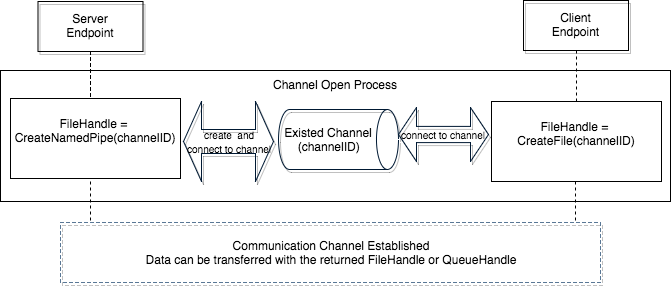
\includegraphics[scale=0.55]{Figures/namepipechannelopen}}
 \caption{Channel Open Process for a Named Pipe}
\label{namedpipeopen}
\end{figure}

\subsection{Message Queue}
Similar to Named Pipe, Message Queue's implementation in Windows also has two modes, synchronous and asynchronous. Moreover, the asynchronous mode further divides into two operations, one with callback function while the other without. With the callback function, the callback function would be called when the send or receive operations finish. Without callback function, the general function \textit{MQGetOverlappedResult} should be called by the endpoints to check if the message sending or receiving operation finish, the output message will be stored in the overlap structure whose memory address saved in the function's output parameter Overlap Structure Address. Table\ref{msmqsynfunctions} lists the functions for synchronous mode while Table\ref{msmqasynfunctionscallback} and Table\ref{msmqasynfunctions} list the functions for the asynchronous mode with and without callback. 

    \begin{table}[H]
        \centering
        \caption{Function List  of events for Synchronous MSMQ}
        \label{msmqsynfunctions}
        \begin{tabular}{|l|l|l|}
            \hline
             \textbf{Event} & \textbf{Function}& \textbf{Parameters}  \\
             \hline
             \multirow{2}{*}{{\textbf{Channel Open}}}
             &\multirow{2}{*}{{MQOpenQueue}} &  RAX: Queue Handler\\
              \cline{3-3} 
             & &  RCX: Queue Format Name\\
            \hline
             \multirow{2}{*}{{\textbf{Send}}}
             &\multirow{2}{*}{MQSendMessage} &  RCX: Queue Handle \\
              \cline{3-3} 
             &&  RDX: Message description structure Address \\
            \hline
             \multirow{2}{*}{{\textbf{Receive}}}
             & \multirow{2}{*}{MQReceiveMessage}&  RCX: Queue Handle \\
              \cline{3-3} 
              &&  R9: Message description structure Address \\
            \hline
            \textbf{Channel Close} &MQCloseQueue & RCX: Queue Handler \\
            \hline
        \end{tabular}
    \end{table}


    \begin{table}[H]
        \centering
        \caption{Function List of events for Asynchronous MSMQ with Callback}
        \label{msmqasynfunctionscallback}
        \begin{tabular}{|l|l|l|}
            \hline
             \textbf{Event} & \textbf{Function}& \textbf{Parameters}  \\
             \hline
             \multirow{2}{*}{{\textbf{Channel Open}}}
             &\multirow{2}{*}{{MQOpenQueue}} &  RAX: Queue Handler\\
              \cline{3-3} 
             & &  RCX: Queue Format Name\\
            \hline
             \multirow{2}{*}{\textbf{Send}}
             &\multirow{2}{*}{MQSendMessage} &  RCX: Queue Handle \\
              \cline{3-3} 
             &&  RDX: Message description structure Address \\
            \hline
             \multirow{2}{*}{\textbf{Receive}}
             & \multirow{2}{*}{MQReceiveMessage}&  RCX: Queue Handle \\
              \cline{3-3} 
              &&  R9: Message description structure Address \\
             \hline
             \textbf{Receive}
              &CallbackFuncName&  Parameters for the callback function. \\
            \hline
            \textbf{Channel Close} &MQCloseQueue & RCX: Queue Handler \\
            \hline
        \end{tabular}
    \end{table}

    \begin{table}[H]
        \centering
        \caption{Function List  of events for Asynchronous MSMQ without Callback}
        \label{msmqasynfunctions}
        \begin{tabular}{|l|l|l|}
            \hline
             \textbf{Event} & \textbf{Function}& \textbf{Parameters}  \\
             \hline
             \multirow{2}{*}{{\textbf{Channel Open}}}
             &\multirow{2}{*}{{MQOpenQueue}} &  RAX: Queue Handler\\
              \cline{3-3} 
             & &  RCX: Queue Format Name\\
            \hline
             \multirow{2}{*}{{\textbf{Send}}}
             &\multirow{2}{*}{MQSendMessage} &  RCX: Queue Handle \\
              \cline{3-3} 
             &&  RDX: Message description structure Address \\
            \hline
             \multirow{2}{*}{{\textbf{Receive}}}
             & \multirow{2}{*}{MQReceiveMessage}&  RCX: Queue Handle \\
              \cline{3-3} 
              &&  R9: Message description structure Address \\
              \hline
              \textbf{Receive} 
              & MQGetOverlappedResult &  RCX: Overlap Structure address  \\
            \hline
            \textbf{Channel Close} &MQCloseQueue & RCX: Queue Handler \\
            \hline
        \end{tabular}
    \end{table}
    
The endpoints of the communication can create the queue or use the existing one. However, both of them have to open the queue before they access it. The handle ID returned by the open queue function will be used later on when messages are being sent or received to identify the queue. Figure\ref{msmqopen} shows the channel set up process for a Message Queue communication.
\begin{figure}[H]
\centerline{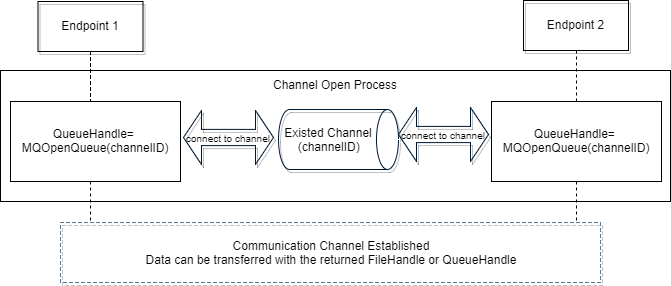
\includegraphics[scale=0.55]{Figures/msmqchannelopen}}
 \caption{Channel Open Process for a Message Queue}
\label{msmqopen}
\end{figure}
    
\subsection{TCP and UDP}
In Windows programming, these two methods shared the same set of APIs regardless the input parameter values and operation behaviour are different. In Windows socket solution, one of the two endpoints is the server while the other one is the client. Table \ref{tcpupdfunctions} lists the functions of a UDP or TCP communication. 
  \begin{table}[H]
        \centering
        \caption{Function List  of events for TCP and UDP}
        \label{tcpupdfunctions}
        \begin{tabular}{|l|l|l|l|l|}
            \hline
             \multirow{2}{*}{\textbf{Event}} &
               \multicolumn{2}{c|}{\textbf{Server Endpoint}} &
               \multicolumn{2}{c|}{\textbf{Client Endpoint}} \\
             \cline{2-5}
              & \textbf{Function}& \textbf{Parameters} & \textbf{Function} & \textbf{Parameters}  \\
             \hline
             \textbf{Channel Open}
             &socket&  RAX: Socket Handle & socket &  RAX: Socket Handle\\
             \hline
                \multirow{2}{*}{{\textbf{Channel Open}}}
              &\multirow{2}{*}{{bind}} &  RCX: Socket Handle & \multirow{2}{*}{connect} &  RCX: Socket Handle\\
              \cline{3-3} \cline{5-5}
             &&  RDX: Server Address $\&$ Port &  &  RDX: Server Address $\&$ Port\\
            \hline
                \multirow{3}{*}{{\textbf{Channel Open}}}
             &\multirow{3}{*}{{accept}} &  RAX: New Socket Handle && \\
              \cline{3-3} 
             &&  RCX:  Socket Handle &  & \\
             \cline{3-3} 
             &&  RDX: Client Address $\&$ Port &  &  \\
            \hline
             \multirow{2}{*}{{\textbf{Send}}}
             &\multirow{2}{*}{send} &  RCX: New Socket Handle & \multirow{2}{*}{send} &  RCX: Socket Handle\\
              \cline{3-3} \cline{5-5}
             &&  RDX: Buffer Address &  &  RDX: Buffer Address\\
           \hline
              \multirow{2}{*}{{\textbf{Receive}}}
             & \multirow{2}{*}{recv}&  RCX: New Socket Handle & \multirow{2}{*}{recv} &  RCX: Socket Handle\\
              \cline{3-3} \cline{5-5}
              &&  RDX: Buffer Address &  &  RDX: Buffer Address\\
            \hline
          {{\textbf{Channel Close}}}&
            {closesocket} & {RCX: New Socket Handle} &{closesocket} & {RCX: Socket Handle}\\
            \hline
        \end{tabular}
    \end{table} 
    
The communication channel is set up by both of the endpoints. The function \textit{socket} should be called to create their own socket on both endpoints. After the sockets are created, the server endpoint binds the socket to its service address and port by calling the function \textit{bind}. Then the server endpoint calls the function  \textit{accept} to accept the client connection. The client will call the function \textit{connect} to connect to the server. When the function \textit{accept} return successfully, a new socket handle will be generated and returned for further data transfer between the server endpoint and  the connected client endpoint. After all these operations are performed successfully, the channel is established and the data transfer can start. During the channel open stage, server endpoint has two socket handles, the first one is used to listen to the connection from the client, while the second one is created for real data transfer. Figure\ref{channelopen2} shows the channel open process for TCP and UDP.
    
\begin{figure}[H]
\centerline{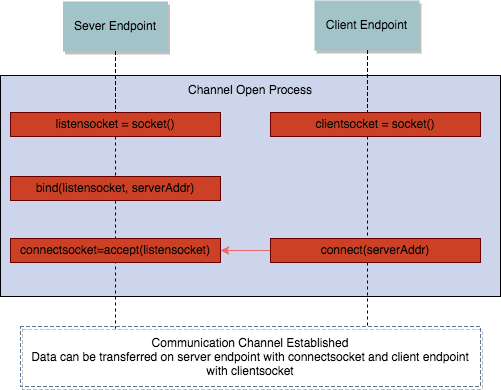
\includegraphics[scale=0.55]{Figures/tcpudpchannelopen}}
 \caption{Channel Open Model for TCP and UDP}
\label{channelopen2}    
\end{figure}


\section{Event Locating Algorithm: $eventfilter\left( \right)$}
The concerned events in a communication are channel open, channel close, send and receive events. These events are identified as system function calls in this work.  A function call in the trace starts from the function call instruction to the function return instruction. The input parameters' value and input buffer content should be retrieved from the memory state of the the function call instruction line while the return value, output parameters' value and output buffer content should be retrieved from the memory state of the function return instruction line. Tables in section \ref{windows} indicate all the functions of the communication methods as well as the concerned parameters. Following the windows calling convention, the concerned parameter value or buffer address can be found in the corresponding register or stack positions. The buffer content can be found in the memory address in the reconstructed memory state. Each event can be completed by different function calls. For example, for the client endpoint in TCP communication method, both  \textit{socket} and \textit{connect} function call are considered to be the channel open events. The functions list for a communication method is needed as a input of this algorithm. Tables in Section\ref{windows} give the examples of function list of the events for some communication methods. The algorithm presented in this section is designed for locating all function calls provided in the function list as events of one communications method. If more than one communication methods are being investigated, this algorithm should be run multiple times, each for a method. Events in the output event list is sorted by time of occurrence. Since the function list usually contain a very small number of functions compared to the instruction line number in the execution trace, the time complexity of this algorithm is O(N+M) , N and M are the instruction line numbers of the two traces in the duel-trace.

\begin{algorithm}[H]
\DontPrintSemicolon
\caption{{\bf Event Locating Algorithm} \label{eventLocAlg}}
\KwIn{ $trace, funcset$}
\KwOut{$event\_trace$}
$event\_trace \leftarrow List \langle Event\rangle$;\; 
\While{not at end of trace}{
   \For{$f \in funcset$}{
       \If{Is function call of f}{ 
           $event.funN = f.funN$
           $event.startline \leftarrow$ current Line number;\;
           $event.endline \leftarrow$ find function return instruction line;\;          
           $event.inputs \leftarrow$ reconstruct memory of $event.startline$ from the trace and get input values of $f.pars$;\;              
           $event.outputs \leftarrow$ reconstruct memory of $event.endline$ from the trace and get outputs values of $f.pars$;\;
           $event.type \leftarrow f.type$;\;
           $event\_trace.add\left( event \right)$;\;
       }       
    }
}
\KwRet $event\_trace$;\;
\end{algorithm} 

\section{Stream Identification Algorithm: $streamfilter\left( \right)$}
The events located in the $event\_trace$ may correspond to different $stream$, the next step in the communication identification algorithm is to identify them for each $stream$. The input of this algorithm the $event\_trace$ from the ``Event Locating Algorithm". Since the input  $event\_trace$ is sorted by time of occurrence and the channel open events should always happen before other events, it is reasonable to assume the new stream can be identified by its first channel open function call. The identification for TCP and UDP server endpoints are slightly complicated than the other ones, due to its own channel open mechanism. The output of this algorithm is the $stream\_trace$. Each stream in this $stream\_trace$ consist of the sub streams. The concepts of the stream and sub streams are defined in Section\ref{term}. 

\begin{algorithm}[H]
\DontPrintSemicolon
\caption{{\bf Stream Indentification Algorithm} \label{endpointIdentAlg}}
\KwIn{$event\_trace$}
\KwOut{$stream\_trace$}
$stream\_trace \leftarrow Map \langle String, List \langle EndPoint\rangle \rangle$;\; 
\For{$event \in event\_trace$}{
   \If{$event$ is a channel open event}{
      $handle \leftarrow$ get the handle identifier from the function parameter list;\;
      $stream \leftarrow stream\_trace.get\left( handle \right)$;\;
      \If{$event$ is an $accept\left( event \right)$ function call for TCP or UDP}{
         $newHandle \leftarrow$ get the second socket handle identifier which is the return value from the function parameter list;\;
         $stream\_trace.remove\left( handle \right)$;\;
         $stream\_trace.add\left( newHandle, endpoint \right)$;\;
      }
      
      \If{$endpoint$ is null}{
         $stream = New \enspace Stream\left( \right)$;\;
         $stream\_trace.add\left( hanele, endpoint \right)$;\;
      }
      $stream.openStream.add\left( event \right)$;\;
   }
   \If{$event$ is a channel send event}{
      $handle \leftarrow$ get the handle from the function parameter list;\;
      $stream \leftarrow stream\_trace.get\left( handle \right)$;\;
      \If{$stream$ is not $null$ and $stream.complete$ is $False$}{
         $stream.sendStream.add\left( event \right)$;\;
      }
   }
   \If{$event$ is a channel receive event}{
      $handle \leftarrow$ get the handle from the function parameter list;\;
      $stream \leftarrow stream\_trace.get\left( handle \right)$;\;
      \If{$stream$ is not $null$ and $stream.complete$ is $False$}{
         $stream.receiveStream.add\left( event \right)$;\;
      }
   }
   \If{$event$ is a channel close event}{
      $handle \leftarrow$ get the handle from the function parameter list;\;
      $stream \leftarrow stream\_trace.get\left( handle \right)$;\;
      \If{$stream$ is not null}{
         $stream.closeStream.add\left( event \right)$;\;
         $stream \leftarrow True$;\;
      }
   }         
}
\KwRet $stream\_trace$;\;
\end{algorithm} 

\section{Stream Matching Algorithm: $streammatch()$}\label{streammatch}
The communication identification algorithm aims at identifying all the communication of a concerned communication method from the dual-trace. The input of this algorithm is the two $stream\_trace$ from the dual-trace. The output of this algorithm is the communication list. Each communication recognized from the dual\_trace contains two $stream$s. The channel of a communication defined in Section\ref{definition} is not explicitly represented in the output but it was implicitly used in this algorithm. 

In the communication identification algorithm, it first try to match two $stream$s to a channel only by their identifiers. In this level, the matching depends on channel open mechanisms which are different from communication method to communication method. For TCP and UDP the matching can be considered as local address and port of server endpoint matching with remote address and port of client endpoint. For Named Pipe, it uses the file name, while for Message Queue, it uses the queue name as the identifier for matching of two endpoints. 

The first level matching can not guarantee the exact endpoints matching and channel identification. There are two situations which false negative error might emerge. Take Named Pipe for example, the first situation is multiple(more than two) interacting programs shared the same file or queue as their own channel. Even though the channels are distinct for each communication, but the file or queue used is the same one. For example, the Named Pipe server is connected by two clients using the same file. In the server trace, there are two $stream$s found. In each client trace, there is one $stream$ found. For the dual\_trace of server and client1, there will be two possible identified communications, one is the real communication for server and client1 while the other is the false negative error actually is for server and client2. The $stream$ in client1's trace will be matched by two $stream$s in the server's trace. The second situation is the same channel is reused by the different endpoints in the same programs. For example, the Named Pipe server and client finished the first communication and then closed the channel. After a while they re-open the same file again for another communication. Since the first level matching is only base on the identifiers and the first and the second communications have the same identifier since they used the same file. Similar situations can also happen in Message Queue, TCP and UDP communication methods. 

To reduce the false negative error, the second level matching should be applied, which is also being named as transmitted data verification algorithm. On top of the endpoint identifiers matching, further data verification should be applied to make sure the matching is reliable. This verification crossly compare the sent and received data in both $stream$s in the first level matching. If the transmitted data in the $stream$s are considered to be identical, the matching is confirmed, otherwise it was a false negative error. However, we still can not exclude all the false negative errors, due to the data transmitted in two communication can be identical. Figure\ref{secondlevelmatching} indicates the ineffective second level matching scenario and the effective one.

\begin{figure}[H]
\centerline{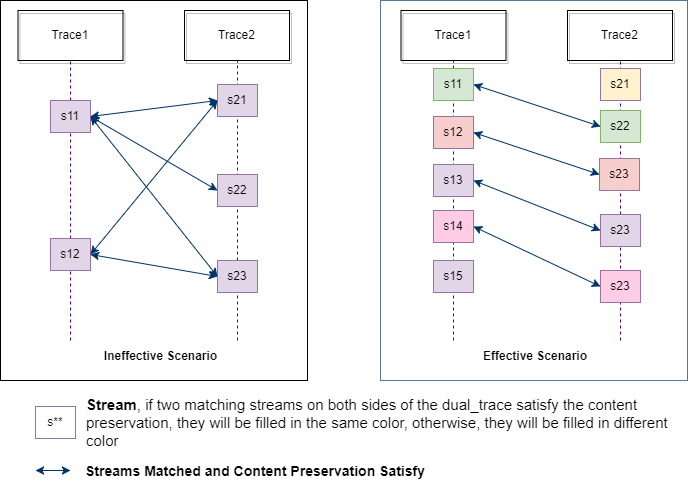
\includegraphics[scale=0.55]{Figures/secondlevelmatching}}
 \caption{Second Level Matching Scenarios}
\label{secondlevelmatching}
\end{figure}


The following subsections discuss the algorithms for these two level matching. In Section\ref{windows}, I elaborate the channel open process and the data transfer categories for the concerned communication methods. Based on the different channel opening process, two algorithms are developed for the communication identification, one is for Named Pipe and Message Queue, the other is for TCP and UDP. The inputs of the these two algorithms are the same, two $stream\_trace$s from the original dual\_trace.

The data transfer characteristics divided the communication methods into reliable and unreliable transmissions. Named Pipe and TCP fall in the reliable category while Message Queue and UDP fall in the unreliable one. The second level matching algorithms are different for these two categories. The corresponding second level data verification algorithms are being used in the communication identification algorithms. The inputs of the transmitted data verification algorithms are $stream$s matched in the first level matching while the output a boolean to indicate if the transmitted data of this two $stream$s are matched and the verified data.

\subsection{Stream Matching Algorithm for Named Pipe and Message Queue}
For Named Pipe and Message Queue, only one channel open function is being called in each $stream$. So in the below algorithm, when it try to get the channel open event from the $stream.openStream$ list, only one event should be found and return. The channel identifier parameters can be found in the $event.inputs$ of the channel open event. The identifier for Named Pipe is the file name of the pipe while for Message Queue is the format queue name of the queue. This algorithm finds out all the possible communications regardless some of them might be false negative errors. 

\begin{algorithm}[H]
\DontPrintSemicolon
\caption{{\bf Stream Matching Algorithm for Named Pipe and Message Queue} \label{channelAlg1}}
\KwIn{$stream\_trace_{0}, stream\_trace_{1}$}
\KwOut{$cos = \left\lbrace co_{y}: 0\leqslant y \leqslant Y\right\rbrace $}
$cos \leftarrow Map \langle String, List \langle Communication \rangle \rangle$;\; 
\For{$stream0 \in stream\_trace_{0}$}{
   $openEvent0 \leftarrow$ get the opening event from $stream0.openStream$;\;
   $channelId0 \leftarrow$ get the channel identifier from $openEvent0.inputs$;\;
   \For{$stream1 \in stream\_trace_{1}$}{
      $openEvent1 \leftarrow$ get the opening event from $stream1.openStream$;\;
      $channelId1 \leftarrow$ get the channel identifier from $openEvent1.inputs$;\;
     \If{$channelId0 == channelId1$}{
         $DataVerified = dataVerify(stream0, stream1, outputdata)$;\;
         \If{$DataVerified == True$}{
            $communication = New \enspace Communication()$;\;
            $communication.stream0 = stream0$;\;
            $communication.stream1 = stream1$;\;
            $communication.dataMatch = outputdata$;\;
            $cos.add\left( communication \right)$;\;
         }    
      }
   }
}
\KwRet $cos$;\;
\end{algorithm} 


\subsection{Stream Matching Algorithm for TCP and UDP}
For TCP and UDP multiple functions are collaborating to create the final communication channel. The local address and port of the server endpoint and the remote address and port of the client endpoint are used to identify the channel. This algorithm first try to retrieve the local address and port of the server endpoint and remote address and port from client endpoint. Then it try to match two endpoints by comparing the local and remote address and port. Transmitted data verification also applied in this algorithm.

\begin{algorithm}[H]
\DontPrintSemicolon
\caption{{\bf Stream Matching Algorithm for TCP and UDP} \label{channelAlg2}}
\KwIn{$stream\_trace_{0}, stream\_trace_{1}$}
\KwOut{$cos = \left\lbrace co_{y}: 0\leqslant y \leqslant Y\right\rbrace $}
$cos \leftarrow Map \langle String, List \langle Communication \rangle \rangle$;\; 
\For{$stream0 \in stream\_trace_{0}$}{
   $socketEvent0 \leftarrow$ get the $socket\left( \right)$ event from $stream0.openStream$;\;
   $bindEvent0 \leftarrow$ get the $bind\left( \right)$ event from $stream0.openStream$;\;
   $connectEvent0 \leftarrow$ get the $connect\left( \right)$ event from $stream0.openStream$;\;
   \For{$stream1 \in stream\_trace_{1}$}{
      $socketEvent1 \leftarrow$ get the $socket\left( \right)$ event from $stream1.openStream$;\;
      $bindEvent1 \leftarrow$ get the $bind\left( \right)$ event from $stream1.openStream$;\;
      $connectEvent1 \leftarrow$ get the $connect\left( \right)$ event from $stream1.openStream$;\;
    \If{$socketEvent0 !=null$ AND $socketEvent1 != null$}{
       \If{$bindEvent0 != null$ AND $connectEvent1 == null$}{
           $localServerAddr \leftarrow$ get serverAddr from $bindEvent1.inputs$;\;
       }
       \ElseIf{$bindEvent1 == null$ AND $connectEvent0 != null$}{
           $remoteServerAddr \leftarrow$ get serverAddr from $connectEvent1.inputs$;\; 
       }
       \Else{
          Break the inner For loop;\;
       }
       \If{$localServerAddr == remoteServerAddr$}{
          $DataVerified = dataVerify(stream0, stream1, outputdata)$.
          $communication = New \enspace Communication()$;\;
          $communication.stream0 = stream0$;\;
          $communication.stream1 = stream1$;\;
          $communication.dataMatch = outputdata$; 
          $cos.add\left( communication \right)$;\;
       }
    }
   }
}
\KwRet $cos$;\;
\end{algorithm}

\subsection{Data Verification $dataVerify()$ for Named Pipe and TCP}
As described in Section\ref{reliable}, the data being received by one endpoint should always equal to or at least is sub string of the data being sent from the other endpoint in a communication for the reliable transmission methods, such as Named Pipe and TCP. So the data verification algorithm is in data union level. The send data union is retrieved by the concatenation of the input buffer content of the send events in the send stream of an endpoint. The receive data union is retrieved by the concatenation of the output buffer content of the receive events in the receive stream of the other endpoint. The input of this algorithm is the two $stream$s from two traces which are being matched in the first level.

\begin{algorithm}[H]
\DontPrintSemicolon
\caption{{\bf Transmitted Verification by Data Union} \label{dataAlg1}}
\KwIn{$stream0, stream1$}
\KwOut{send data union and receive data union of two streams}
\KwRet{Indicator of if transmitted data union are considered to be identical}
$send1 \leftarrow$ empty string;\;
$send2 \leftarrow$ empty string;\;
$recv1 \leftarrow$ empty string;\;
$recv2 \leftarrow$ empty string;\;
\For{$sendEvent \in stream0.sendStream$}{
   $sendmessage \leftarrow$ get the input buffer content from the $sendEvent.inputs$;\;
   $send0.append\left( sendmessage \right)$;\;
}
\For{$sendEvent \in stream1.sendStream$}{
   $sendmessage \leftarrow$ get the input buffer content from the $sendEvent.inputs$;\;
   $send1.append\left( sendmessage \right)$;\;
}
\For{$recvEvent \in stream0.receiveStream$}{
   $recvmessage \leftarrow$ get the output buffer content from the $recvEvent.outputs$;\;
   $recv0.append\left( sendmessage \right)$;\;
}
\For{$recvEvent \in stream1.receiveStream$}{
   $recvmessage \leftarrow$ get the output buffer content from the $recvEvent.outputs$;\;
   $recv1.append\left( sendmessage \right)$;\;
}
\If{$recv0$ is substring of $send1$ AND $recv1$ is substring of $send0$ }{
   \KwRet True;\;
}
\Else{
    \KwRet False;\;
}

\end{algorithm} 

\subsection{Data Verification $dataVerify()$ for MSMQ and UDP}
For the unreliable communication methods, the data packets being transmitted are not delivery and ordering guaranteed. So it is impossible to verify the transmitted data as a whole chunk. Fortunately, the packets arrived to the receivers are always as the original one from the sender. Therefore, we perform the transmitted data verification by single events instead of the whole stream. This algorithm basically goes through $event$s of the $sendstream$ in one $stream$ trying to find the matched receive event in the $receivestream$ in the other $stream$. And then calculate the fail packet arrival rate. The fail packet arrival rate should be comparable to the packet lost rate. So we set the packet lost rate as the threshold to determine if the transmitted data can considered to be identical in both directions. The packet lost rate can be various from network to network or even from time to time for the same network. The inputs of this algorithm are the copies of two $stream$s from two traces which are being matched and the packet lost rate as the threshold. I use copies instead of original data is to modify the input list directly in the algorithm. The threshold should be an integer. For example if the lost rate is 5\%, the threshold should be set as 5. 

\begin{algorithm}[H]
\DontPrintSemicolon
\caption{{\bf Transmitted Verification by Data of Events } \label{dataAlg2}}
\KwIn{$stream0, stream1$}
\KwOut{matched event list of two endpoints}
\KwRet{Indicator of if transmitted data union are considered to be identical}
$sendPktNum0 \leftarrow stream0.sendStream.length$;\;
$sendPktNum1 \leftarrow stream1.sendStream.length$;\;
$recvPktNum0 \leftarrow 0$;\;
$recvPktNum1 \leftarrow 0$;\;
$eventMatchs \leftarrow List \langle EventMatch \rangle$;\;
\For{$sendEvent \in stream0.sendStream$}{
   $sendmessage \leftarrow$ get the input buffer content from the $sendEvent.inputs$;\;
   \For{$recvEvent \in stream1.receiveStream$}{
      $recvmessage \leftarrow$ get the output buffer content from the $recvEvent.outputs$;\;
      \If{$sendmessage == recvmessage$}{
         $recvPktNum0++$;\;
         $stream1.receiveStream.remove\left( recvEvent \right)$;\;
         $eventMatch = New eventMatch\left( \right)$;\;
         $eventMatchs.add\left( eventMatch \right)$;\;
      }
   }
}

\If{$ \left(sendPktNum0-recvPktNum0\right)*100/sendPktNum0 > threshold$}{
 \KwRet False;\;
}

\For{$sendEvent \in stream1.sendStream$}{
   $sendmessage \leftarrow$ get the input buffer content from the $sendEvent.inputs$;\;
   \For{$recvEvent \in stream0.receiveStream$}{
      $recvmessage \leftarrow$ get the output buffer content from the $recvEvent.outputs$;\;
      \If{$sendmessage == recvmessage$}{
         $recvPktNum1++$;\;
         $stream0.receiveStream.remove\left( recvEvent \right)$;\;
      }
   }
}

\If{$ \left(sendPktNum1-recvPktNum1\right)*100/sendPktNum1 > threshold$}{
 \KwRet False;\;
}
 \KwRet True;\;
\end{algorithm}



\section{Data Structures for Identified Communications}
In the previous sections, I elaborate all the essential algorithms to identify the communications. The information of identified communications should be organized properly for the further presentation or visualization to the user. In this section, I define the output data structures to fulfil this requirement. There are totally two major data set. The first one is clustered as communications aligning the definition at Section\ref{definition}. The second one is clustered by endpoints in the traces. The reason to provide the second data set is due to the false negative errors of the channel identification. The identified endpoint lists of the traces provide more original data information. So with other assistant information and the access of this relatively original information of the dual-trace, the user has more flexibility to analysis the dual-trace. The data structures have been used in the algorithms implicitly.

\begin{algorithm}[H]
\DontPrintSemicolon
\caption{{\bf Data Structure for Identified Communications} \label{communicationlData}}
$communications \leftarrow Map \langle String, List \langle Communication \rangle \rangle$;
$stream\_traces \leftarrow Map \langle String, List \langle Stream \rangle \rangle$;  
\Struct{Communication}{
  Stream stream0 \tcp*[f]{stream0 is from $trace_{0}$ of the dual-trace}\;  
  Stream stream1 \tcp*[f]{stream1 is from $trace_{1}$ of the dual-trace}\;  
  DataMatch dataMatch\;  
}


\Union{DataMatch}{
  DataUnionMatch \quad  unionMatch \tcp*[f]{For data union verification}\;  
  List $\langle$ EventMatch $\rangle$ \enspace eventMatchs \tcp*[f]{For data event verification}\;  
}

\Struct{DataUnionMatch}{
  String sData1 \tcp*[f]{send data union of endpoint1}\;  
  String rData1 \tcp*[f]{receive data union of endpoint1,substring of sData2}\;  
  String sData2 \tcp*[f]{send data union of endpoint2}\;  
  String rData2 \tcp*[f]{receive data union of endpoint2,substring of sData1}\; 
}

\Struct{EventMatch}{
  Event \quad \quad event1 \tcp*[f]{event1 is from enpoint1}\;  
  Event \quad \quad event2 \tcp*[f]{event2 is from enpoint2}\;  
}


\Struct{Stream}{
  Int \quad \quad handle\;
  List $\langle$ Event $\rangle$ \enspace openStream\;
  List $\langle$ Event $\rangle$ \enspace closeStream\;
  List $\langle$ Event $\rangle$ \enspace sendStream\;
  List $\langle$ Event $\rangle$ \enspace receiveStream\; 
}

\Struct{Event}{
   Int \quad \quad \quad \quad \quad \quad \quad \quad stratline\;
   Int \quad \quad \quad \quad \quad \quad \quad \quad endline\;
   Map $\langle$ String, String $\rangle$ \enspace inputs\; 
   Map $\langle$ String, String $\rangle$ \enspace outputs\; 
}

\end{algorithm} 